\chapter{Implementation}\label{chap:5}
%EXPERIMENTAL RESULTS AND ANALYSIS
%
%
\section{Environment}
\section{Over view}
Our system use machine learning technique, known as decision tree algorithm for malware classification system. Our goal is fast malware classification and we use decision tree algorithm to achieve that goal. Classification is a form of supervised learning, which requires training data, with known input/output, to form knowledge \cite{tonylee}. As shown in Figure \ref{fig:system_architec}, Our system contains three parts.\\
\begin{itemize}
\item First part: Read binary file to take meta data and input to database.\\
\item Second part: Manually cluster malware which load from database.\\
\item Third part: Use decision tree algorithm to classify malware.\\
\end{itemize}
\begin{figure}[h!]
\centering
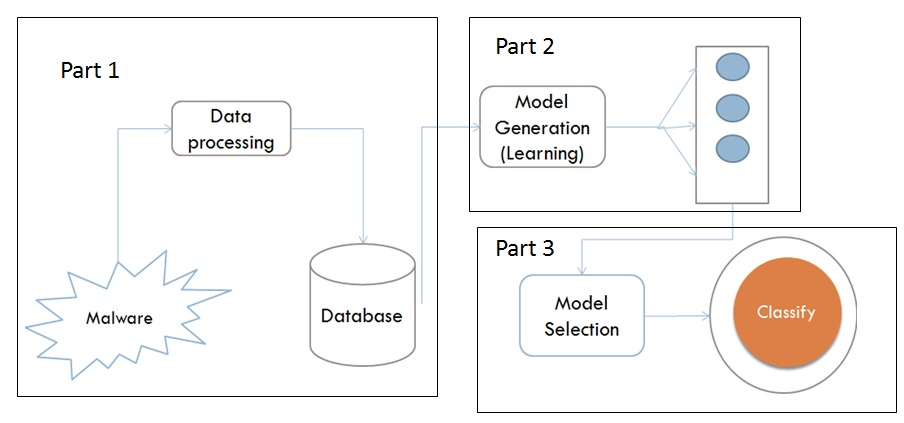
\includegraphics[width=1\textwidth]
{graph/system_architec1.jpg}
\caption{The system architecture.}
\label{fig:system_architec}
\end{figure}
We want to analyse a vast amount of malware so our system use database to store malware file's meta-data, to easily control a vast amount of data and easily share in the internet by web browser.
The flow of data is shown in the Figure \ref{fig:system_architec}. We read binary file meta-data and input all of the meta-data in to database. In the second part, our system export meta-data in database as the training data to create the decision tree for classifying malware. Lastly, we use the decision tree algorithm which created in the second part to classify unknown malware into the different malware families. 
%CLASSFICATION BASE ON DECISION TREE
%
%
\section{Classification based on machine learning technique} 
\subsection{Meta-data}
In order to create a fast malware classification system, we only use PE header's meta-data to classify malware. PE header includes meta-data of MS-DOS section, COFF file header, Optional header, and Section header.\\
There is a problem that PE file's meta data value is so large that it is very difficult to detect unknown malware which have meta-data's different to the training data of our system. We index meta-data of PE header file which have semantic information for malware classification. For example, normally \emph{ImageBase} field of PE header file have value 400000h \cite{goppit} so that the value of ImageBase of malware file in our system is 0 if it has 40000h and it is 1 if it has other value, and in this research we call that value is semantic value. In this approach, all of PE file's meta-data is used. For example, consist of \emph{HeaderFilesize}, \emph{AddressOfEntryPoint}, \emph{Sizeofsection}, \emph{Imagebase}, \emph{Numberofsection}, \emph{StackCommit}, \emph{SizeHeap Commit}, \emph{SizeImage}, \emph{Characteristics}. We calculated the semantic value of all malware file's meta-data.
\subsection{Create training data}
Virustotal is a service that analyzes malware and facilitates quick collection of viruses, worms, trojans, and all kinds of malware detected by antivirus vendor such as Norton and Kaspersky \cite{virustotal}. In this research, we use virustotal service to take the name of malware provided by Kaspersky and use it in order to cluster malware into malware families which have semantic information. 
We use http post technique to automatically get name from virus total service and cluster malware into malware families which shown in Figure \ref{fig:familymalware}.
\begin{figure}[h!]
\centering
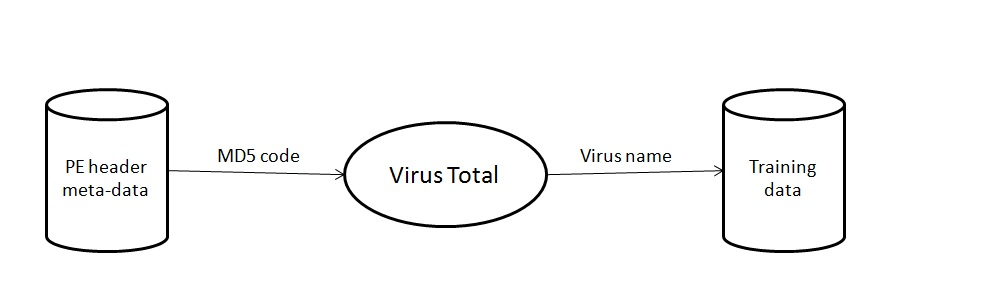
\includegraphics[width=1\textwidth]{graph/clustering.jpg}
\caption{Clustering method.}
\label{fig:clustering}
\end{figure}
\newline
\subsection{Classification}
\begin{figure}[h!]
\centering
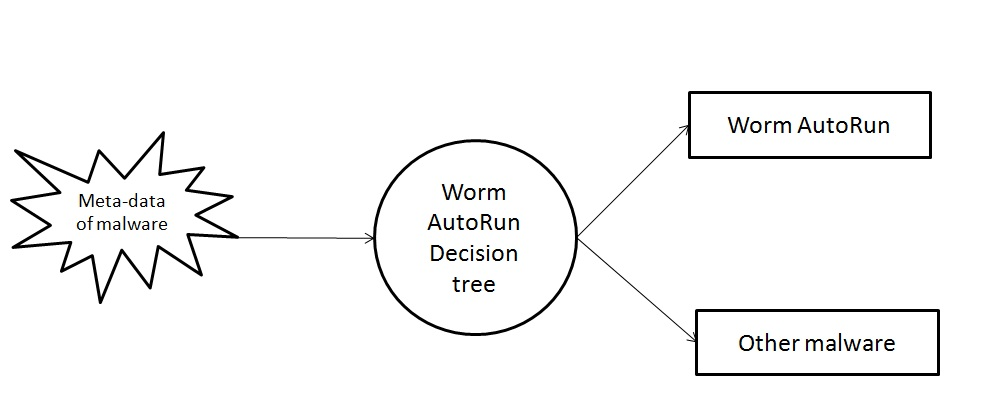
\includegraphics[width=1\textwidth]{graph/classificationdecision.jpg}
\caption{Worm autorun decision tree.}
\label{fig:classificationdecision}
\end{figure}
To make malware classification rapid and correct, we use decision tree algorithm. We make the malware classification which easy to update a new malware family, our classification use decision tree algorithm to determine each malware family. For example, based on training data taken from clustering part, we create six decision trees. In the worm autorun decision tree, shown in Figure \ref{fig:classificationdecision}.\\
We use malware' meta-data as input data for each decision tree, and the the decision tree determine that the malware belongs to worm autorun family or not. If the input malware belong to worm autorun then malware classification detect the family that malware belong to, else we continue to the next decision tree. We use list malware PE header file's meta-data :Magic, MajorLinkerVersion, MinorLinkerVersion, SizeOfCode, SizeOfInitializedData, SizeOfUninitializedData, AddressOfEntryPoint, BaseOfCode, BaseOfData, ImageBase, SectionAlignment, FileAlignment, MajorOperatingSystemVersion, MinorOperatingSystemVersion, MajorImageVersion, MinorImageVersion, MajorSubsystemVersion, MinorSubsystemVersion, Reserved1, SizeOfImage, SizeOfHeaders, CheckSum, Subsystem, DllCharacteristics, SizeOfStackReserve, SizeOfStackCommit, SizeOfHeapReserve, SizeOfHeapCommit, LoaderFlags, NumberOfRvaAndSizes, Machine, NumberOfSections, TimeDateStamp, PointerToSymbolTable, NumberOfSymbols, SizeOfOptionalHeader, Characteristics. A value of each field in PE header have semantic for decision tree algorithm if it is appeared at 10\% in malware training data. With this approach, we created the list semantic value of meta-data of malware. For example, this is list meta-data we created :1, 2, 6, 4, 0, 1, 1, 4, 0, 200, 4, 0, 0, 0, 4, 0, 0, 1.00E+00, 200, 0, 2, 0, 100000, 4000, 100000, 1000, 0, 10, 14c, 2, 1000, 8, 0, e0, 3, 818e. This is value before we calculated :35328, 10b, 2, 0, 6200, 0, 200, b32e, b000, 9000, 400000, 1000, 200, 3, 0, 0, 0, 4, 0, 0, d000, 400, afe8, 2, 0, 1000, 1000, 10000, 0, 0, 10, 14c, 6, 0, 0, 0, e0, 10e. 
Our malware classification part is shown in Figure \ref{fig:classification}. A training data taken from the malware clustering part is used to create the order of decision tree that make malware classification system correct.
The decision tree we created, shown in Figure \ref{fig:decisiontreeworm}. PE header's meta-data of malware is inputted into the worn autorun decision tree in order to determine unknown malware. Then, the malware is determined belongs to worm auto run family or not.\\
\begin{figure}[h!]
\centering
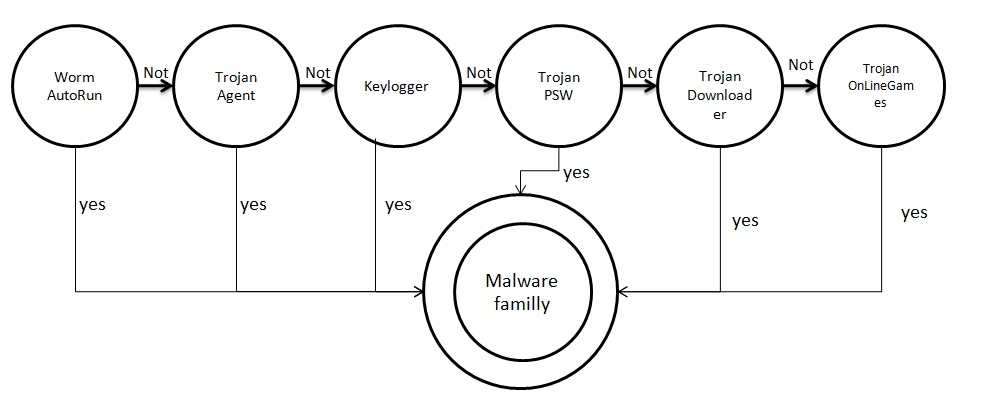
\includegraphics[width=1\textwidth]{graph/classification.jpg}
\caption{Malware classification system.}
\label{fig:classification}
\end{figure}
\begin{figure}[h!]
\centering
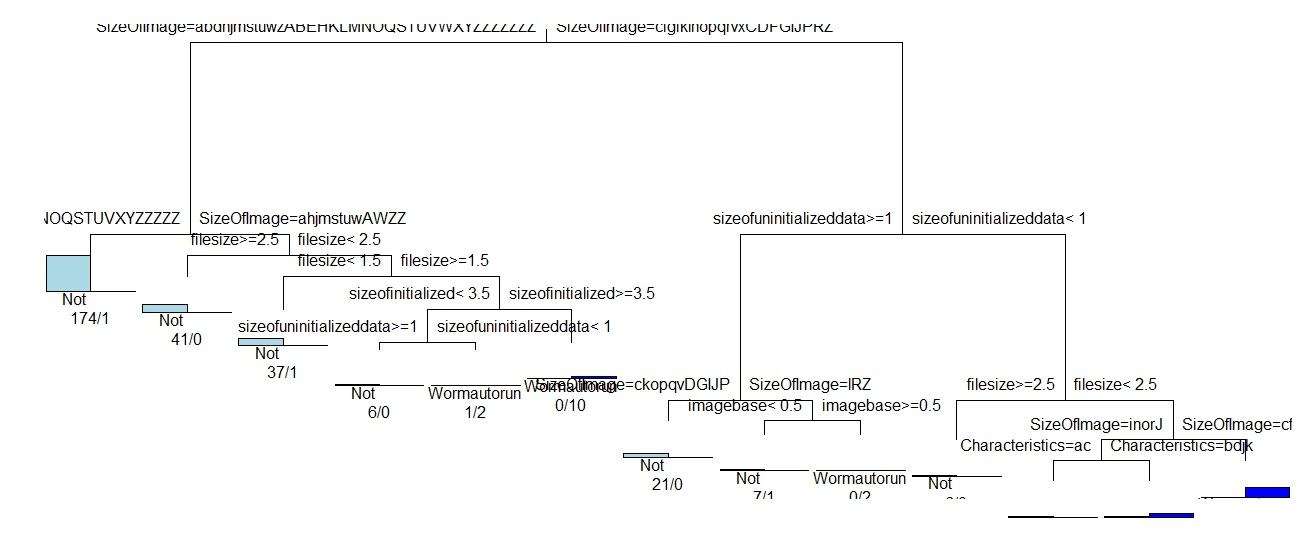
\includegraphics[width=1\textwidth]{graph/decisiontreeworm.jpg}
\caption{Worm autorun decision tree.}
\label{fig:decisiontreeworm}
\end{figure}
